\section{Modalità di esecuzione dei test}
In questa sezione si andrà ad analizzare le performance delle tre soluzioni VPN descritte nei capitoli precedenti, al fine di valutare quale di esse offre le prestazioni migliori.
Le prestazioni verranno valutate analizzando il throughput, la sua stabilità e la percentuale di packetloss.
I software che sono stati utilizzati per effettuare le misurazioni questi dati sono \texttt{iPerf3} e \texttt{mrt}.

\subsection{Panoramica di \texttt{iPerf3}}
\texttt{iPerf} è uno strumento open source che permette di misurare le prestazioni di una rete.
Per effettuare le misurazioni, iPerf crea dei flussi di dati su TCP, UDP o SCTP e invia traffico da un host all'altro; al termine del trasferimento, oltre a un report dettagliato in base al tipo di misurazione richiesta, mostra la larghezza di banda media disponibile.
In questo modo, gli utenti possono determinare il throughput effettivamente utilizzabile.

\begin{figure}[ht]
    \centering
    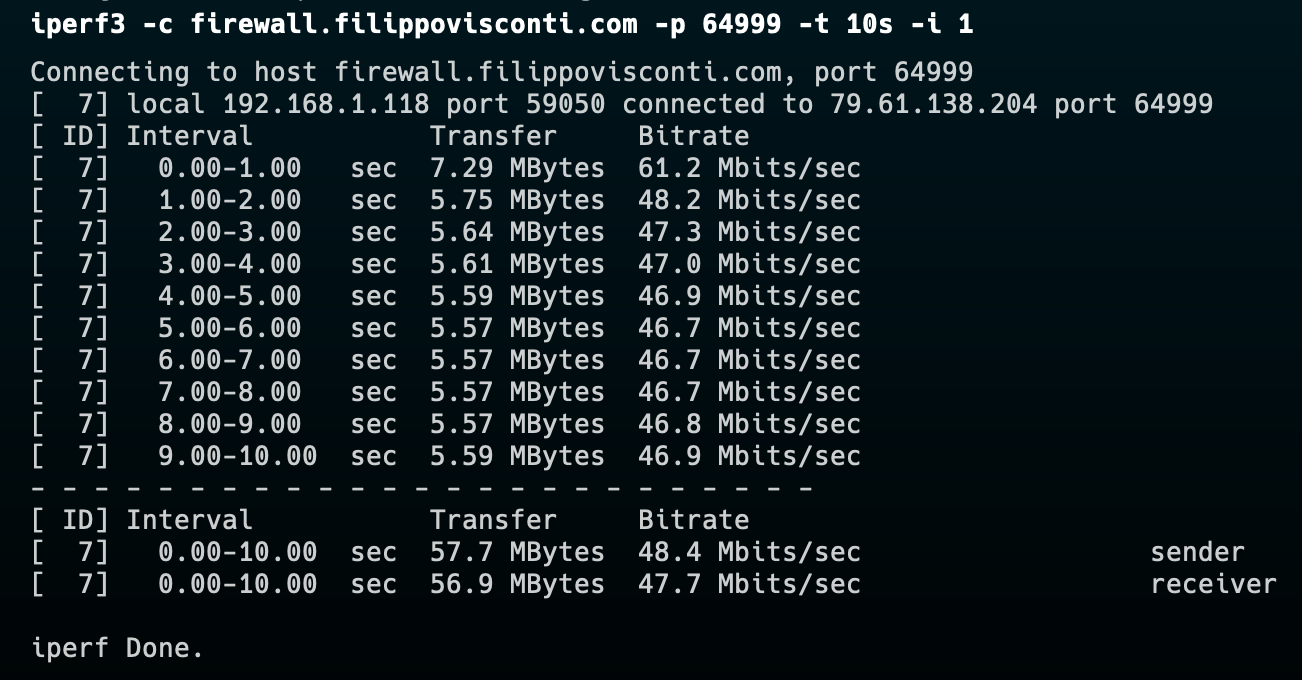
\includegraphics[width=10cm]{figure/iperfSample.png}
    \caption{Esempio di output di iPerf3}
\end{figure}

\subsection{Panoramica di \texttt{mrt}}
\texttt{mtr} è un altro software di misurazione delle performance di una rete, che sostanzialmente unisce i risultati di traceroute e ping.
I test effettuati da mtr sono unidirezionali, dunque è opportuno effettuare misurazioni manualmente in entrambe le direzioni, in quanto i risultati differire in maniera sostanziale. Per avere una misurazione affidabile, è consigliabile far durare il test almeno 10 minuti.

\begin{figure}[ht]
    \centering
    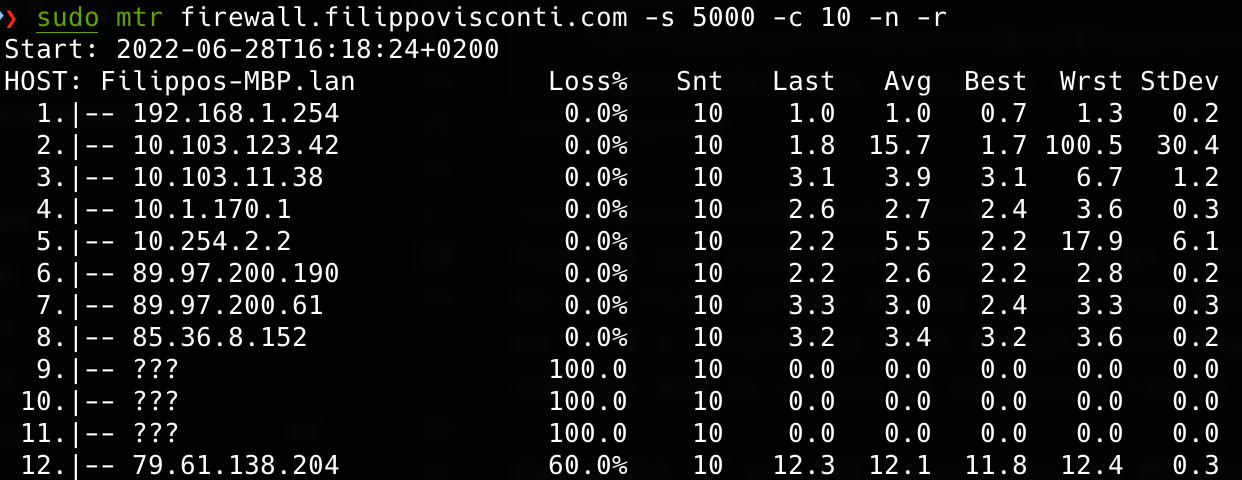
\includegraphics[width=10cm]{figure/mtrSample.png}
    \caption{Esempio di output di mrt}
\end{figure}

\subsubsection{Spiegazione del formato dell'output}
Nella prima colonna, si legge un numero e un indirizzo IP: il numero corrisponde alla distanza in hop tra l'host da cui parte il test e l'IP indicato alla sua destra.
La seconda colonna, \texttt{Loss\%}, indica la percentuale di pacchetti che quell'IP ha perso. È auspicabile un valore inferiore all'1\% per una connessione affidabile.
La terza colonna, \texttt{Snt}, indica il numero di pacchetti inviati a quell'IP.
Le successive 4 colonne indicano il valore dell'ultimo, del medio, del migliore e del peggiore round-trip-time in millisencondi - ossia il tempo necessario affinché un pacchetto parta dal mittente, raggiunga il destinatario, e torni indietro.
L'ultima colonna indica la deviazione standard tra questi ultimi 4 valori.
I valori dalla terza colonna in poi forniscono dunque informazioni sulla latenza della rete. È desiderabile il valore più basso possibile. Tuttavia,  spesso la latenza dipende da fattori esterni alla rete locale.

\subsubsection{Packet loss}
Nella misurazione di esempio, è stato richiesto l'invio di 10 pacchetti (\texttt{-c 10}) di dimensione 5000 byte (\texttt{-s 5000})
On the first column of the report, for each Hop, the percentage of packages that have not reached the destination host is indicated. If in the report we find a single Hop with a high percentage of lost packets this certainly does not represent a network problem. It is generally observed at the ISP address and is caused by bandwidth limits set by the ISP itself or by the fact that the router CPU is busy.

Bandwidth of our ISP causes, on the Mtr report, the presence of a small packet loss in the first hops. These data are very often observable but do not indicate malfunctions or network problems.

A significant loss of data from hop 8 to 13 indicates a serious connection problem and certainly deserves further investigation.

\subsubsection{Latenza}
Network latency:

The latency data is shown in the last five columns of the report (the second column shows the progressive number of the ICMP packets sent). Normally the latency increases proportionally to the test execution time. If the growth is proportional and does not present significant jumps, this means that there are no problems on the network. They do not indicate anomalies nor peak values on the single node 6.

Conversely, if from node 8 onwards high latency values are found (compared to the first 6 hops), which persist until the last hops, it could indicate the presence of numerous problems on the network, such as inadequate configurations of network cards or routers , abnormally working services or network congestion.

\subsection{Scelta della configurazione di test}
Ancora del testo

\subsection{Criteri di valutazione}
Ancora del testo

\subsubsection{Throughput}
Il throughput di un canale di comunicazione misura la quantità di dati che può essere trasferita tra mittente e destinatario in una data unità di tempo. In ambito reti, si è soliti utilizzare come unità di tempo il secondo e come quantità di dati il bit, o suoi multipli (Kbit, Mbit, Gbit).

So, how do we define throughput? Again, network throughput refers to how much data can be transferred from source to destination within a given timeframe. Throughput measures how many packets arrive at their destinations successfully. For the most part, throughput capacity is measured in bits per second, but it can also be measured in data per second.

Packet arrival is key to high-performance service within a network. When people use programs or software, they want their requests to be heard and responded to in a timely fashion. Packets lost in transit lead to poor or slow network performance, and low throughput indicates problems like packet loss. Using throughput to measure network speed is good for troubleshooting because it can root out the exact cause of a slow network and alert administrators to problems specifically in regard to packet loss.

Packet loss, latency, and jitter are all related to slow throughput speed. Latency is the amount of time it takes for a packet to make it from source to destination, and jitter refers to the difference in packet delay. Minimizing all these factors is critical to increasing throughput speed and data performance.

How to Optimize Throughput

By far the most important thing to do when optimizing throughput is to minimize network latency. Latency slows down throughput which, in turn, lowers throughput and delivers poor network performance to users. Generally speaking, you want to minimize lag by monitoring endpoint usage and addressing network bottlenecks.

The most common cause of latency is having too many people trying to use a network at the same time. Latency gets even worse if multiple people are downloading simultaneously. If you’re an IT manager, looking at endpoint usage can tell you which employees are causing latency with non-work-related applications. Even if you’re not an administrator and looking at this from a productivity standpoint, it’s also helpful to know what apps are gumming up the works. Either way, information leads to action.

Network bottlenecks are the IT equivalent of traffic jams. Traffic gets congested for various reasons throughout the day and slows the performance of the network. For example, network performance is typically slow after lunch in large companies because people are returning to their workstations. You can address bottlenecks in many different ways, starting with upgrading routers to keep up with traffic. You can also reduce the number of nodes your network uses, as this will shorten the distance packets have to travel, potentially reducing congestion.
Here are some other tips for reducing latency:

Use a wired connection – Wireless connections can get “lost” because they’re sent through the air. When this happens, servers have to send the information all over again, causing a delay. You can strengthen your wireless signal, but latency is still bound to happen because all wireless signals have this problem to varying degrees. Using an Ethernet cable is a cheap and easy way to improve your connection. Updating to a fiber-optic network is also an option.
Reboot your network – Haven’t turned off your network hardware in a while? It may be causing lag. Unplug the router and modem, wait a few moments, and reboot.
Close applications using up a lot of bandwidth – All network connections have limited bandwidth, and if you’re using more than your fair share, latency will increase. Ease up on those bandwidth-intensive applications.
Disable your firewalls – This may sound like a crazy suggestion at first, but let me explain… Firewalls filter all incoming and outgoing network traffic, and a corrupted firewall can slow your network down. The same will happen if you’re running multiple firewall programs at the same time because they’re both putting tremendous strain on your network. Disabling the firewall can help you figure out if this is a significant factor in your current slowdown.
Go around faulty network hardware – Sometimes lag is caused by faulty hardware. You can try working without certain equipment to see how it affects network speed. Process of elimination will reveal what network hardware, if any, is responsible for latency.
Call in reinforcements – After you’ve run a speed test and checked for packet loss, it may be time to contact your internet service provider. The problem could be on their end.

The network bandwidth definition can be confusing, but basically, network bandwidth is defined as the maximum transfer throughput capacity of a network. It’s a measure of how much data can be sent and received at a time. Bandwidth is measured in bits, megabits, or gigabits per second.

It’s important to know bandwidth doesn’t actually increase the speed of a network, it just appears to make the network faster. You can increase a network’s bandwidth all you want, but all you’ll end up doing is increasing the amount of data that can be sent at one time, not increasing the transmission speed of said data. Bandwidth doesn’t change the speed at which packets are traveling. It’s similarly important to remember high bandwidth doesn’t necessarily equal high network performance. Substantial bandwidth won’t matter if data throughput is still being dragged down by latency, jitter, or packet loss.

Having said this, bandwidth is still important for network speed. Internet speed, for instance, is allocated bandwidth or the amount of data capable of being sent to you per second. For instance, 5 Mbps means you can receive up to five megabits of data per second.

Bandwidth is like a freeway with a strictly enforced speed limit. The cars (data) on the freeway all have to travel at the same speed, so the only way to get more cars on the road, or more data from the internet, is to make the freeway wider. Let’s say 1 Mbps is the equivalent of a single-lane freeway. Let’s also say you want to download a 5 Mb image. If you had a connection with a bandwidth of 1 Mbps (one lane) it would take you about five seconds to download that image.

Now, if you were operating with a 5 Mbps bandwidth connection (five lanes), the same process would take you one second. Here’s the key—your internet connection isn’t any faster from one megabit to the next. What’s different is your data is being transmitted to you at a faster rate because more data can travel down the freeway at the same time. This efficiency makes your internet perceptually faster, not technically faster.

Why is network bandwidth important to administrators, then, if it doesn’t actually increase the speed of their network in any quantifiable way? One of the most important things monitoring bandwidth does is provide information. Administrators need a way to monitor bandwidth, so they can know whether or not they have adequate bandwidth to fit the needs of their applications. Once they have this information and can identify any bandwidth bottlenecks in the system, they can take appropriate steps to rectify the situation—which, in turn, directly increases speed. Monitoring bandwidth availability ensures you would have enough theoretical bandwidth if you ever found yourself in need of it. Using a network monitoring tool allows you to see the actual amount of bandwidth available to your devices and applications within the network.

The difference between bandwidth and throughput isn’t necessarily simple. They tell you two different things about the data in your network, but they’re closely related. You can think of bandwidth as a tube and data throughput as sand. If you have a large tube, you can pour more sand through it at a faster rate. Conversely, if you try to put a lot of sand through a small tube, it will go very slowly.

In short, throughput and bandwidth are two different processes with two different goals both contributing to the speed of a network. Data throughput meaning is a practical measure of actual packet delivery while bandwidth is a theoretical measure of packet delivery. Throughput is often a more important indicator of network performance than bandwidth because it will tell you if your network is literally slow or just hypothetically slow.


\subsubsection{MTU}
A maximum transmission unit (MTU) is the largest packet or frame size, specified in octets (eight-bit bytes) that can be sent in a packet- or frame-based network such as the internet. The internet’s transmission control protocol (TCP) uses the MTU to determine the maximum size of each packet in any transmission. MTU is usually associated with the Ethernet protocol, where a 1500-byte packet is the largest allowed in it (and hence over most of the internet).

One of the most common problems related to MTU is that sometimes higher-level protocols may create packets larger than a particular link supports, and you’ll need to make adjustments to make it work.

To get around this issue, IPv4 allows fragmentation which divides the datagram into pieces. Each piece is small enough to pass over the single link that it is being fragmented for, using the MTU parameter configured for that interface. This fragmentation process takes place at the IP layer (OSI layer 3) and marks the packets it fragments as such. This ensures the IP layer of the destination host knows it should reassemble the packets into the original datagram.

Fragmentation is sometimes not supported by applications, and is something we should avoid if possible. The best way to avoid fragmentation is to adjust the maximum segment size or TCP MSS so the segment will adjust its size before reaching the data link layer.

Before we look at TCP MSS, it helps to understand the build of the  “unit” that’s being sent over the internet.


As mentioned, the common value of MTU in the internet is 1500 bytes.

As you can see in the figure above, the MTU is built from payload (also referred as data) and the TCP and the IP header, 20 bytes each. The total value of the IP and the TCP header is 40 bytes and mandatory for each packet, which leaves us 1460 bytes for our data.

Now, imagine that we are using the GRE protocol in our network, encapsulating the original packet and adding 24 bytes for the GRE header.

The total size of this kind of packet will be 1524 bytes, exceeding the 1500 bytes MTU value. The “data” size in this packet is 1460, but we can and should decrease it in order to make sure the total size will be 1500 bytes or less. And this is where TCP MSS comes into the picture.

TCP MSS, the maximum segment size, is a parameter of the options field of the TCP header that specifies the largest amount of data, specified in bytes, that a computer or communications device can receive in a single TCP segment. It does not include the TCP header or the IP header. This value will dictate the maximum size of the “data” part of the packet. In the following case for the GRE tunnel, we will set the tcp mss value to be 1436 or lower, while the default size is 1460.

The MSS announcement (often mistakenly called a negotiation) is sent during the three-way handshake by both sides, saying: “I can accept TCP segments up to size x”. The size (x) may be larger or smaller than the default. The MSS can be used completely independently in each direction of data flow.

Since the end device will not always know about high level protocols that will be added to this packet along the way, like GRE packets for example, it won’t usually adjust the TCP MSS value. As a result the network devices have the option to rewrite the value of TCP MSS packets that are processed through them. For example, in a Cisco Router the command “ip tcp mss-adjust 1436” in the interface level will rewrite the value of the TCP MSS of any SYN packet that will go via this interface.



\subsubsection{Packetloss}
Quando si accede a Internet o a qualsiasi rete, vengono scambiate delle unità di dati denominate pacchetti. Se uno o più pacchetti non riescono a raggiungere la destinazione prevista, si verifica il fenomeno noto come "perdita di pacchetti". Per gli utenti, la perdita di pacchetti si manifesta sotto forma di interruzioni della rete, servizio lento o anche perdita totale della connettività di rete. Qualsiasi applicazione può essere interrotta dalla perdita di pacchetti, ma le vittime più probabili sono le applicazioni che si affidano all’elaborazione in tempo reale dei pacchetti, come video, audio e giochi.

Le reti aziendali moderne sono alla base delle prestazioni di un’azienda. Se una rete è soggetta a problemi di prestazioni, anche l’azienda ne subisce le conseguenze. Le prestazioni della rete possono essere influenzate da vari problemi operativi, e la perdita di pacchetti è uno dei più comuni. Ma che cos’è la perdita di pacchetti, quale ne è la causa e come può essere prevenuta per garantire che la rete aziendale continui a funzionare al meglio?

The Transmission Control Protocol (TCP) detects packet loss and performs retransmissions to ensure reliable messaging. Packet loss in a TCP connection is also used to avoid congestion and thus produces an intentionally reduced throughput for the connection.

In real-time applications like streaming media or online games, packet loss can affect a user's quality of experience (QoE).
Causes[edit]
The Internet Protocol (IP) is designed according to the end-to-end principle as a best-effort delivery service, with the intention of keeping the logic routers must implement, as simple as possible. If the network made reliable delivery guarantees on its own, that would require store and forward infrastructure, where each router devotes a significant amount of storage space to packets while it waits to verify that the next node properly received them. A reliable network would not be able to maintain its delivery guarantees in the event of a router failure. Reliability is also not needed for all applications. For example, with live streaming media, it is more important to deliver recent packets quickly than to ensure that stale packets are eventually delivered. An application or user may also decide to retry an operation that is taking a long time, in which case another set of packets will be added to the burden of delivering the original set. Such a network might also need a command and control protocol for congestion management, adding even more complexity.

To avoid all of these problems, the Internet Protocol allows for routers to simply drop packets if the router or a network segment is too busy to deliver the data in a timely fashion. This is not ideal for speedy and efficient transmission of data, and is not expected to happen in an uncongested network.[4] Dropping of packets acts as an implicit signal that the network is congested, and may cause senders to reduce the amount of bandwidth consumed, or attempt to find another path. For example, using perceived packet loss as feedback to discover congestion, the Transmission Control Protocol (TCP) is designed so that excessive packet loss will cause the sender to throttle back and stop flooding the bottleneck point with data.

Packets may also be dropped if the IPv4 header checksum or the Ethernet frame check sequence indicates the packet has been corrupted. Packet loss can also be caused by a packet drop attack.

Measurement[edit]
Packet loss may be measured as frame loss rate defined as the percentage of frames that should have been forwarded by a network but were not.[8]

Acceptable packet loss[edit]
Packet loss is closely associated with quality of service considerations. The amount of packet loss that is acceptable depends on the type of data being sent. For example, for voice over IP traffic, one commentator reckoned that "[m]issing one or two packets every now and then will not affect the quality of the conversation. Losses between 5% and 10% of the total packet stream will affect the quality significantly."[9] Another described less than 1% packet loss as "good" for streaming audio or video, and 1–2.5% as "acceptable".[10]

\section{Misure senza VPN}
\begin{figure}[ht]
    \centering
    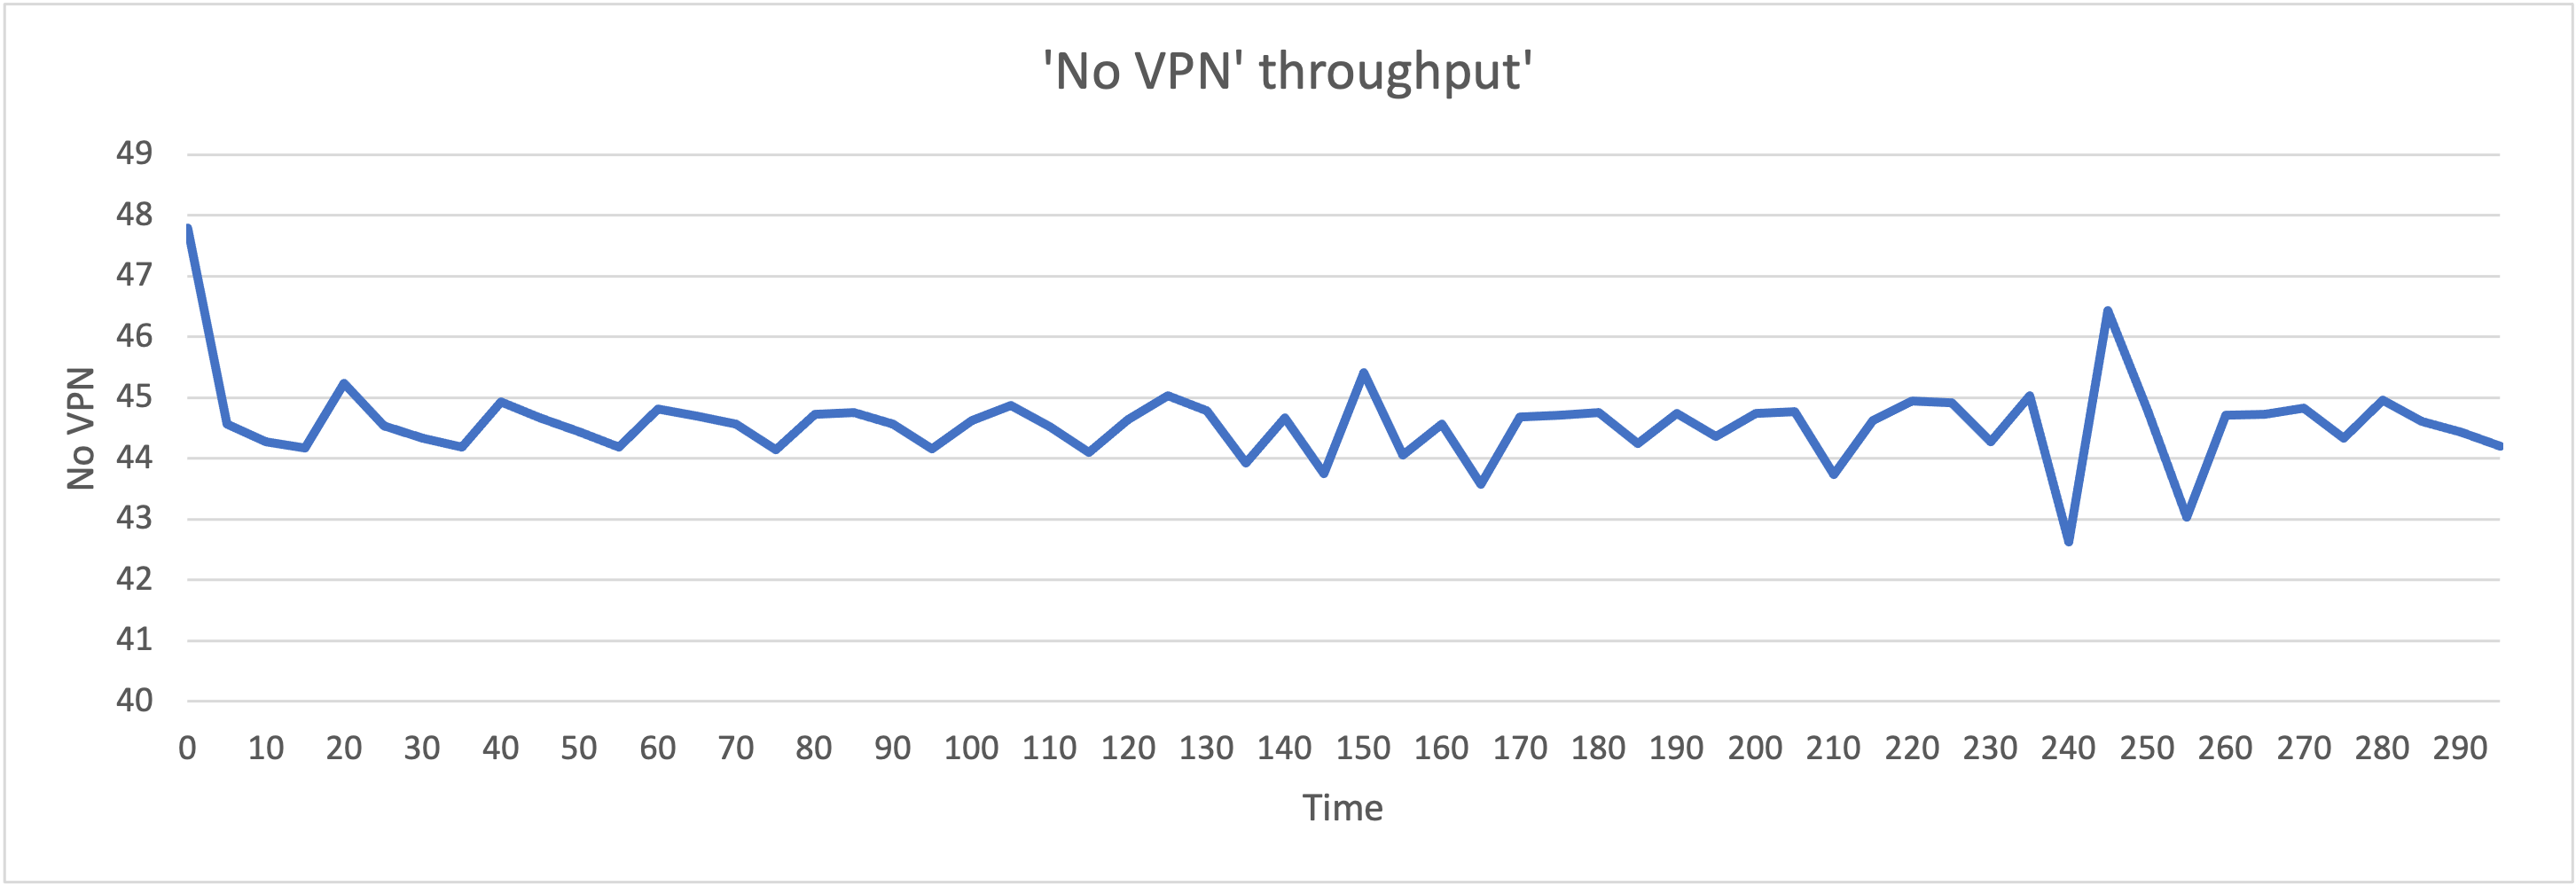
\includegraphics[width=12cm]{figure/vpn_thr.png-1.png}
    \caption{Time in s vs Throughput in Mbit/s}
\end{figure}


\section{Misure con IPSec e IKEv2}
\begin{figure}[ht]
    \centering
    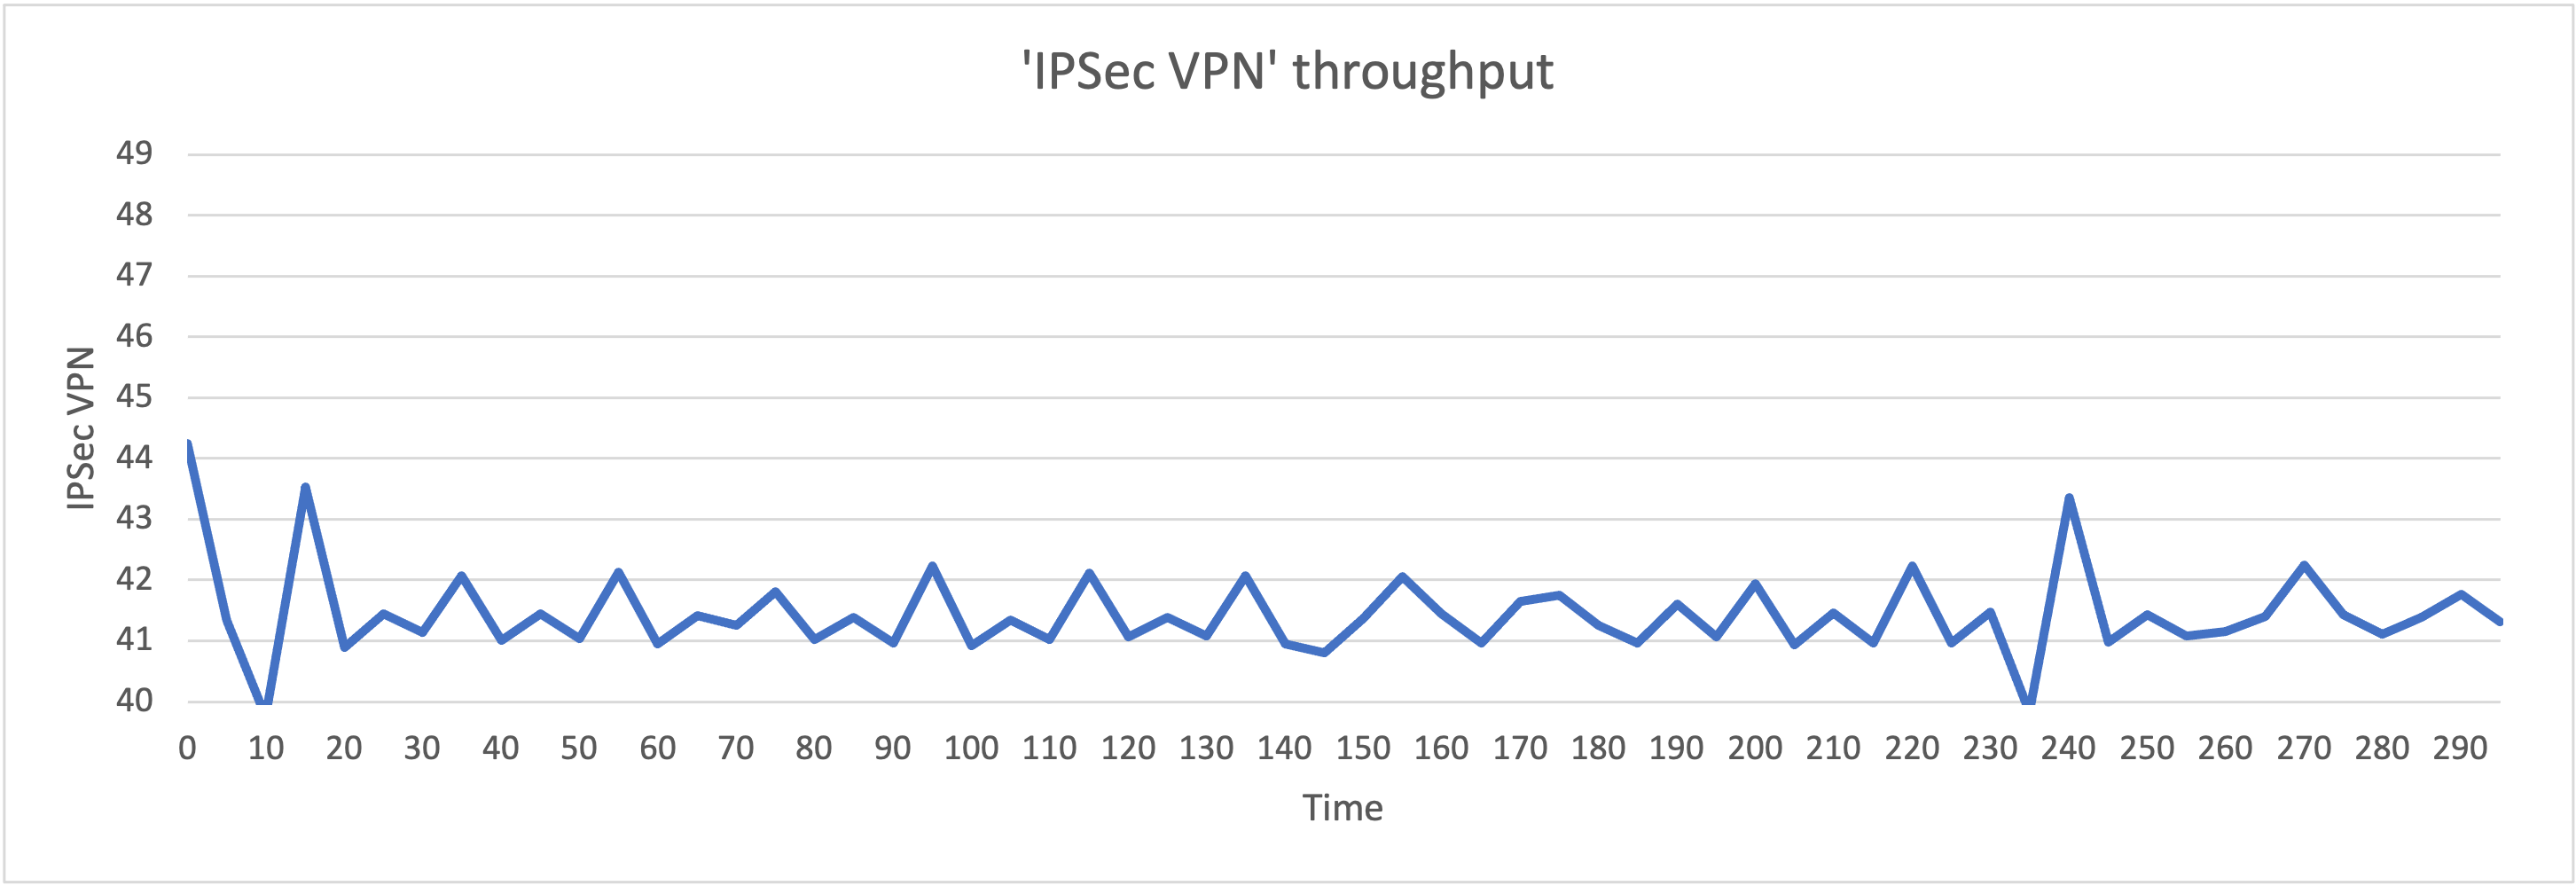
\includegraphics[width=12cm]{figure/vpn_thr.png-2.png}
    \caption{Time in s vs Throughput in Mbit/s}
\end{figure}

\section{Misure con OpenVPN over TCP}
\begin{figure}[ht]
    \centering
    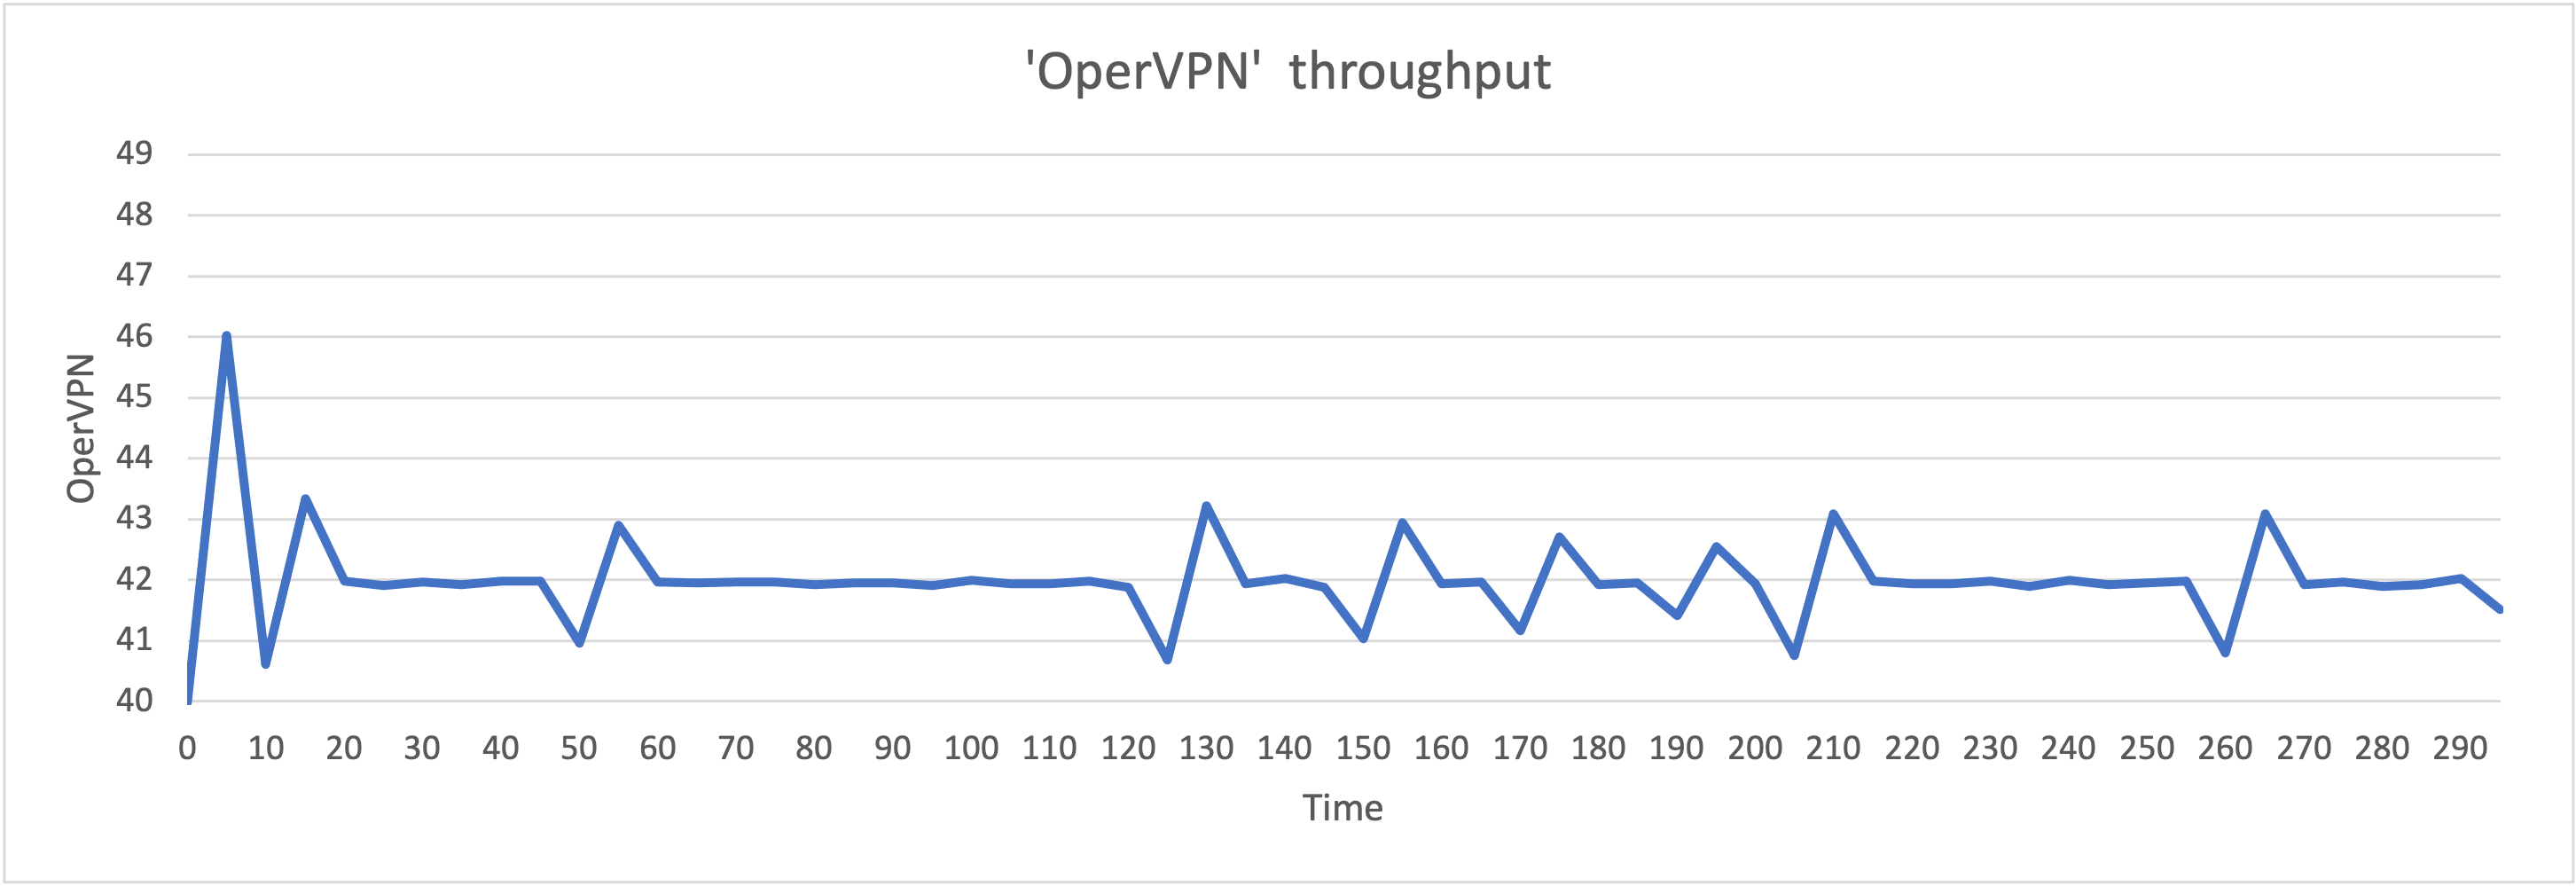
\includegraphics[width=12cm]{figure/vpn_thr.png-3.png}
    \caption{Time in s vs Throughput in Mbit/s}
\end{figure}

\section{Misure con WireGuard}
\begin{figure}[ht]
    \centering
    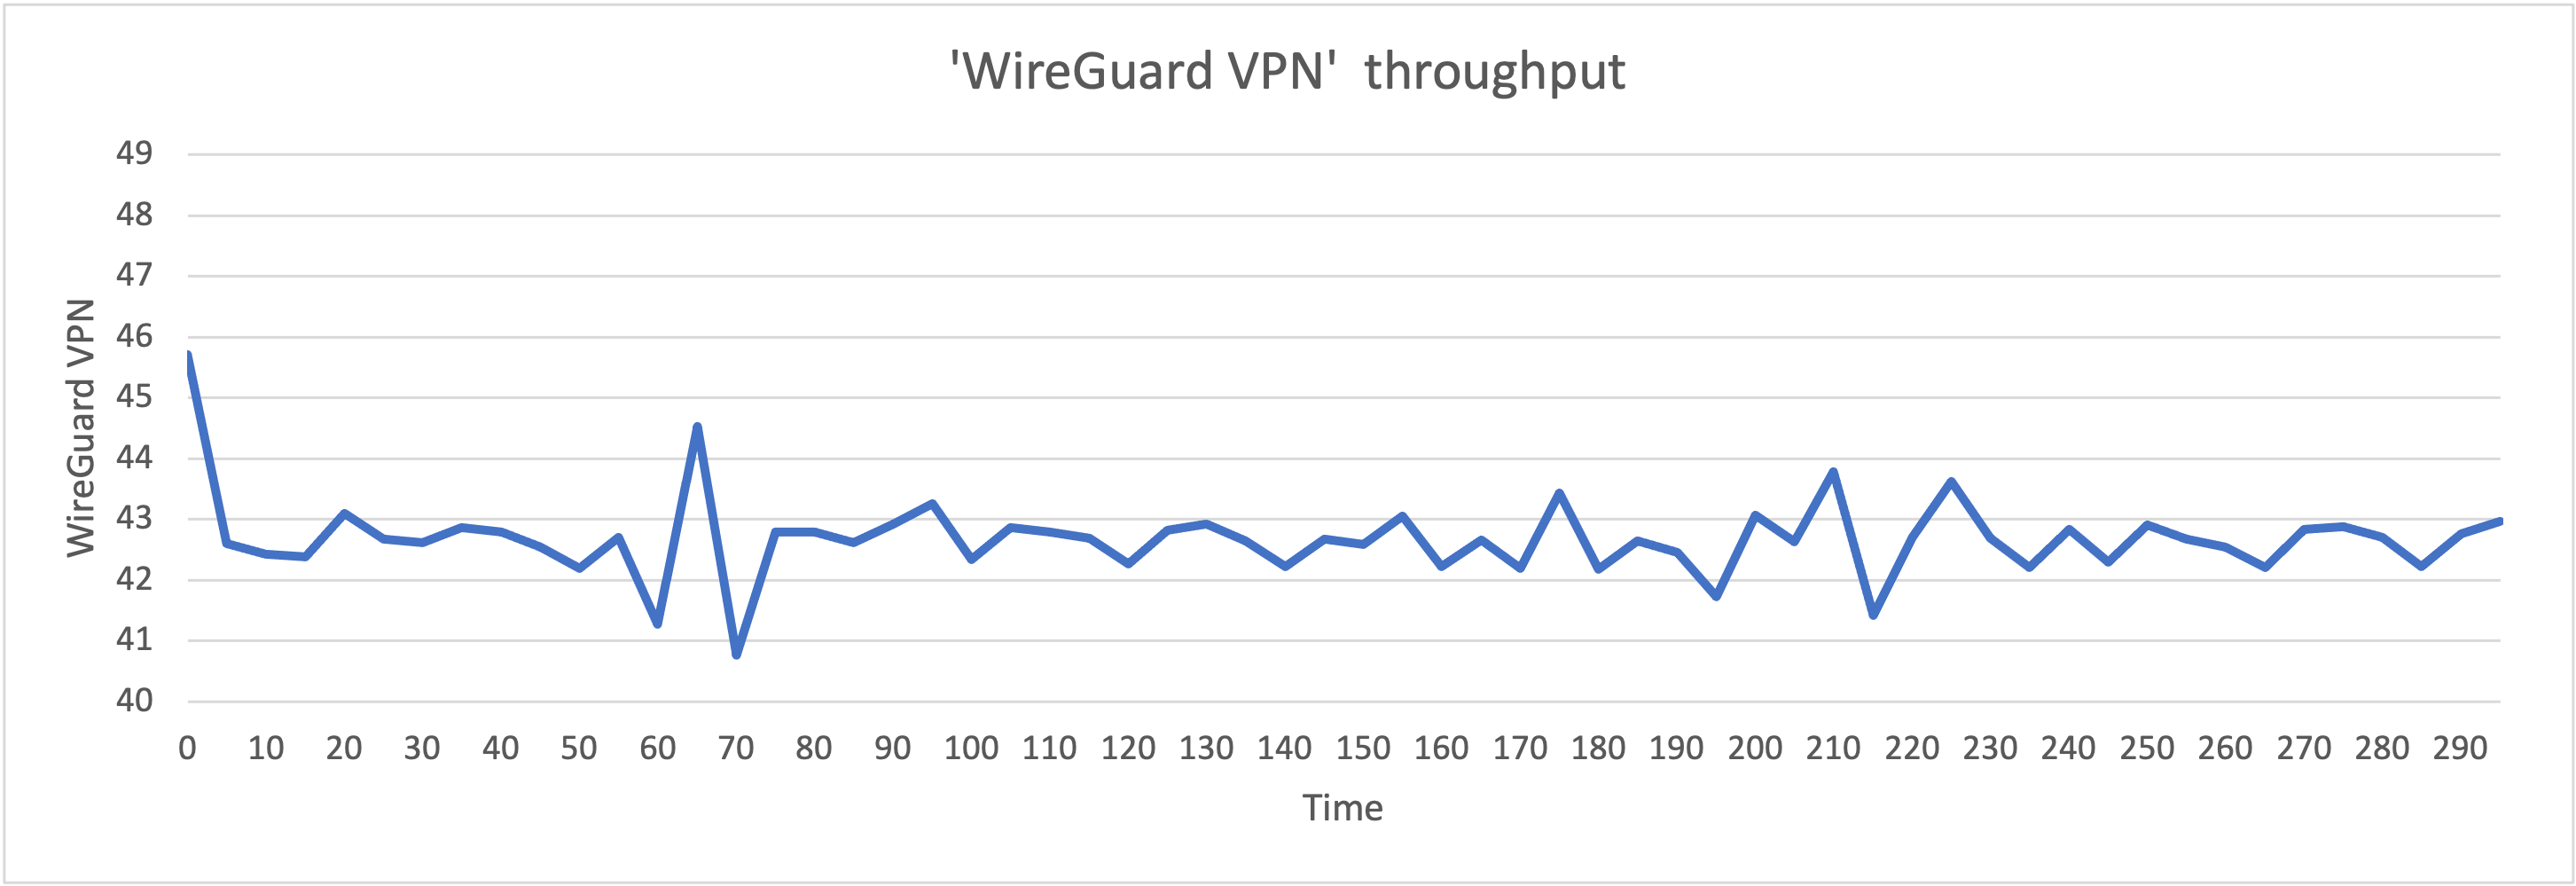
\includegraphics[width=12cm]{figure/vpn_thr.png-4.png}
    \caption{Time in s vs Throughput in Mbit/s}
\end{figure}

\section{Analisi delle misure}
\begin{figure}[ht]
    \centering
    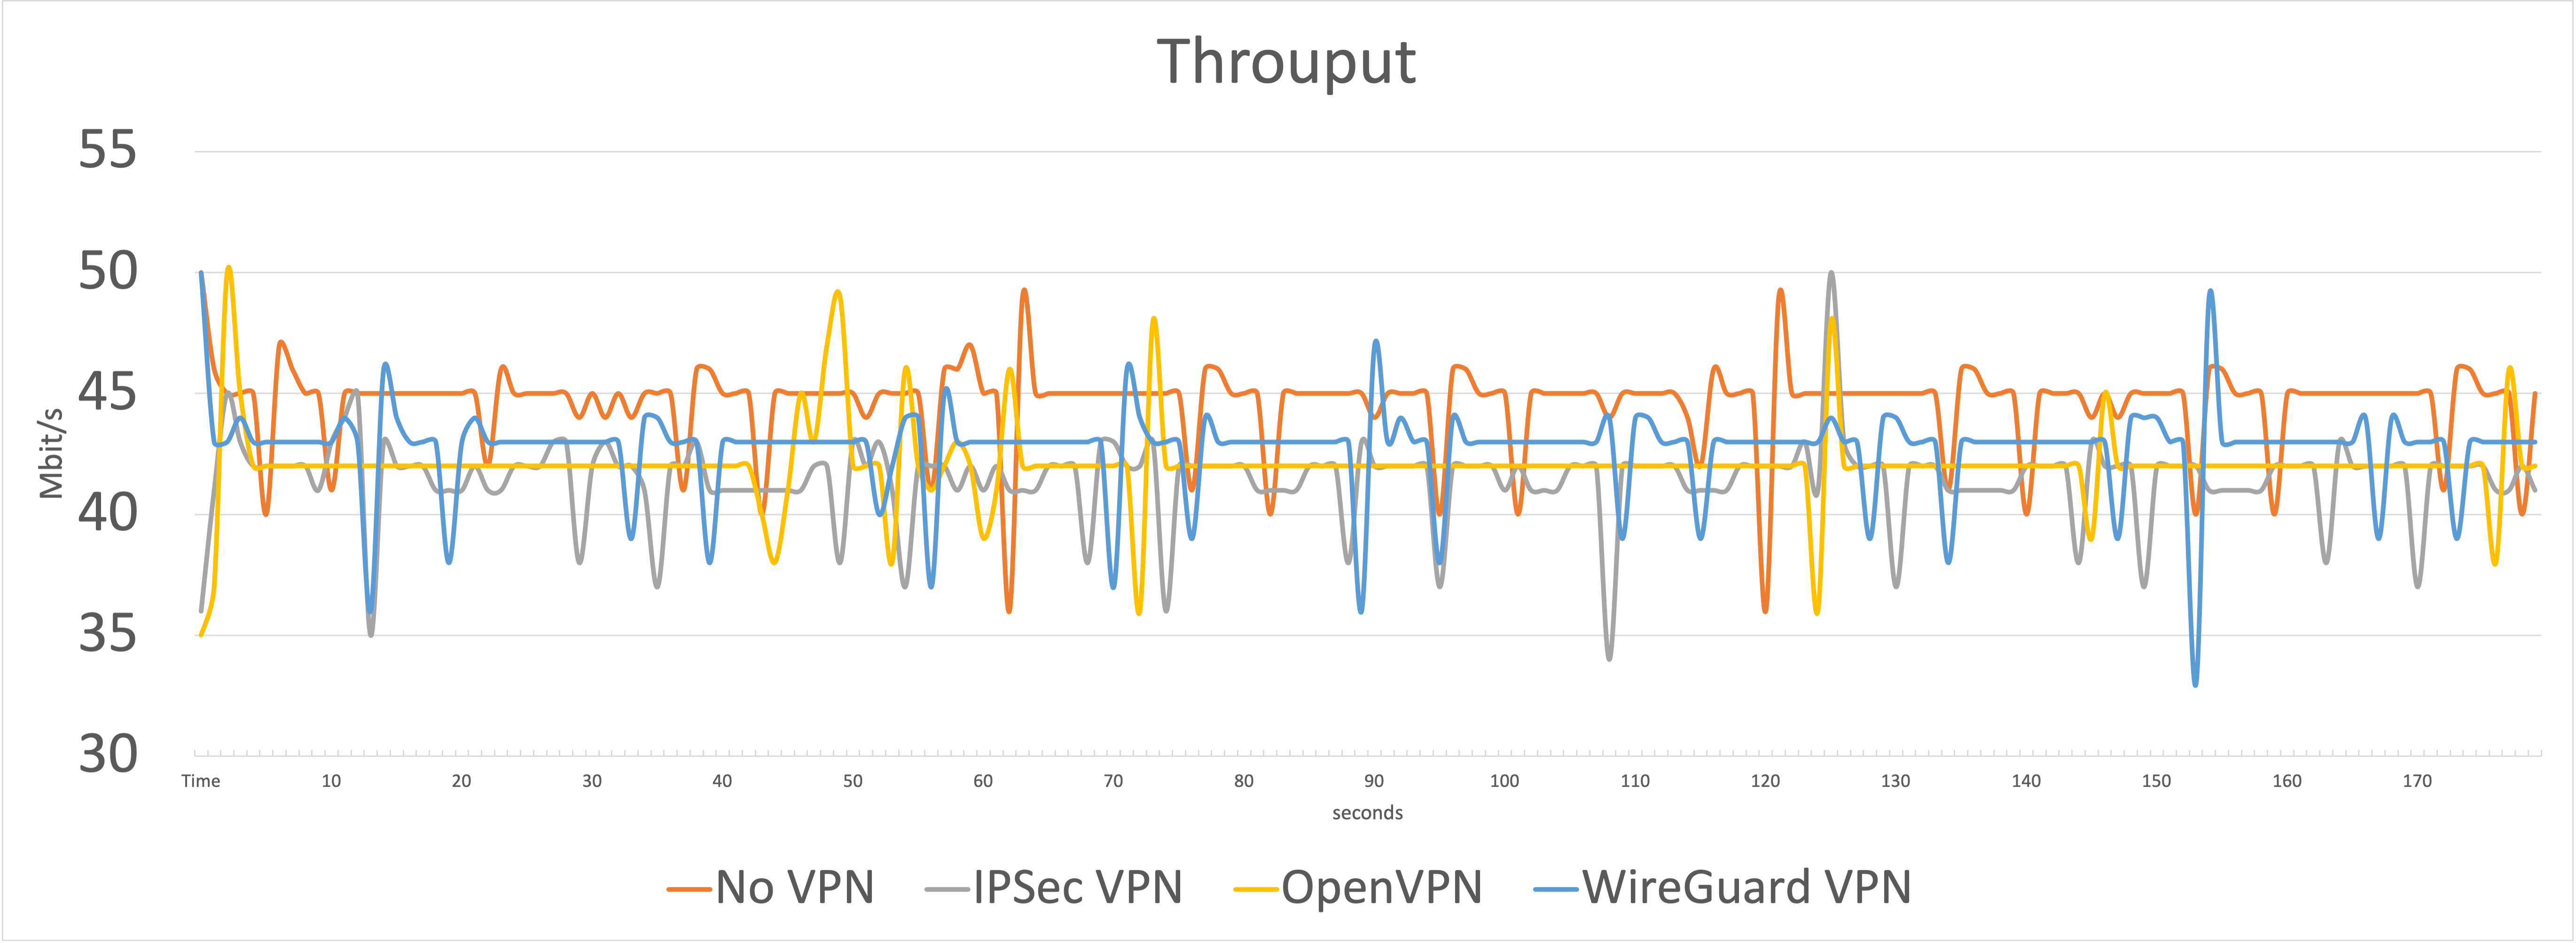
\includegraphics[width=14cm]{figure/rawThroughput.png}
    \caption{Confronto dei throughput grezzi}
\end{figure}

\begin{figure}[ht]
    \centering
    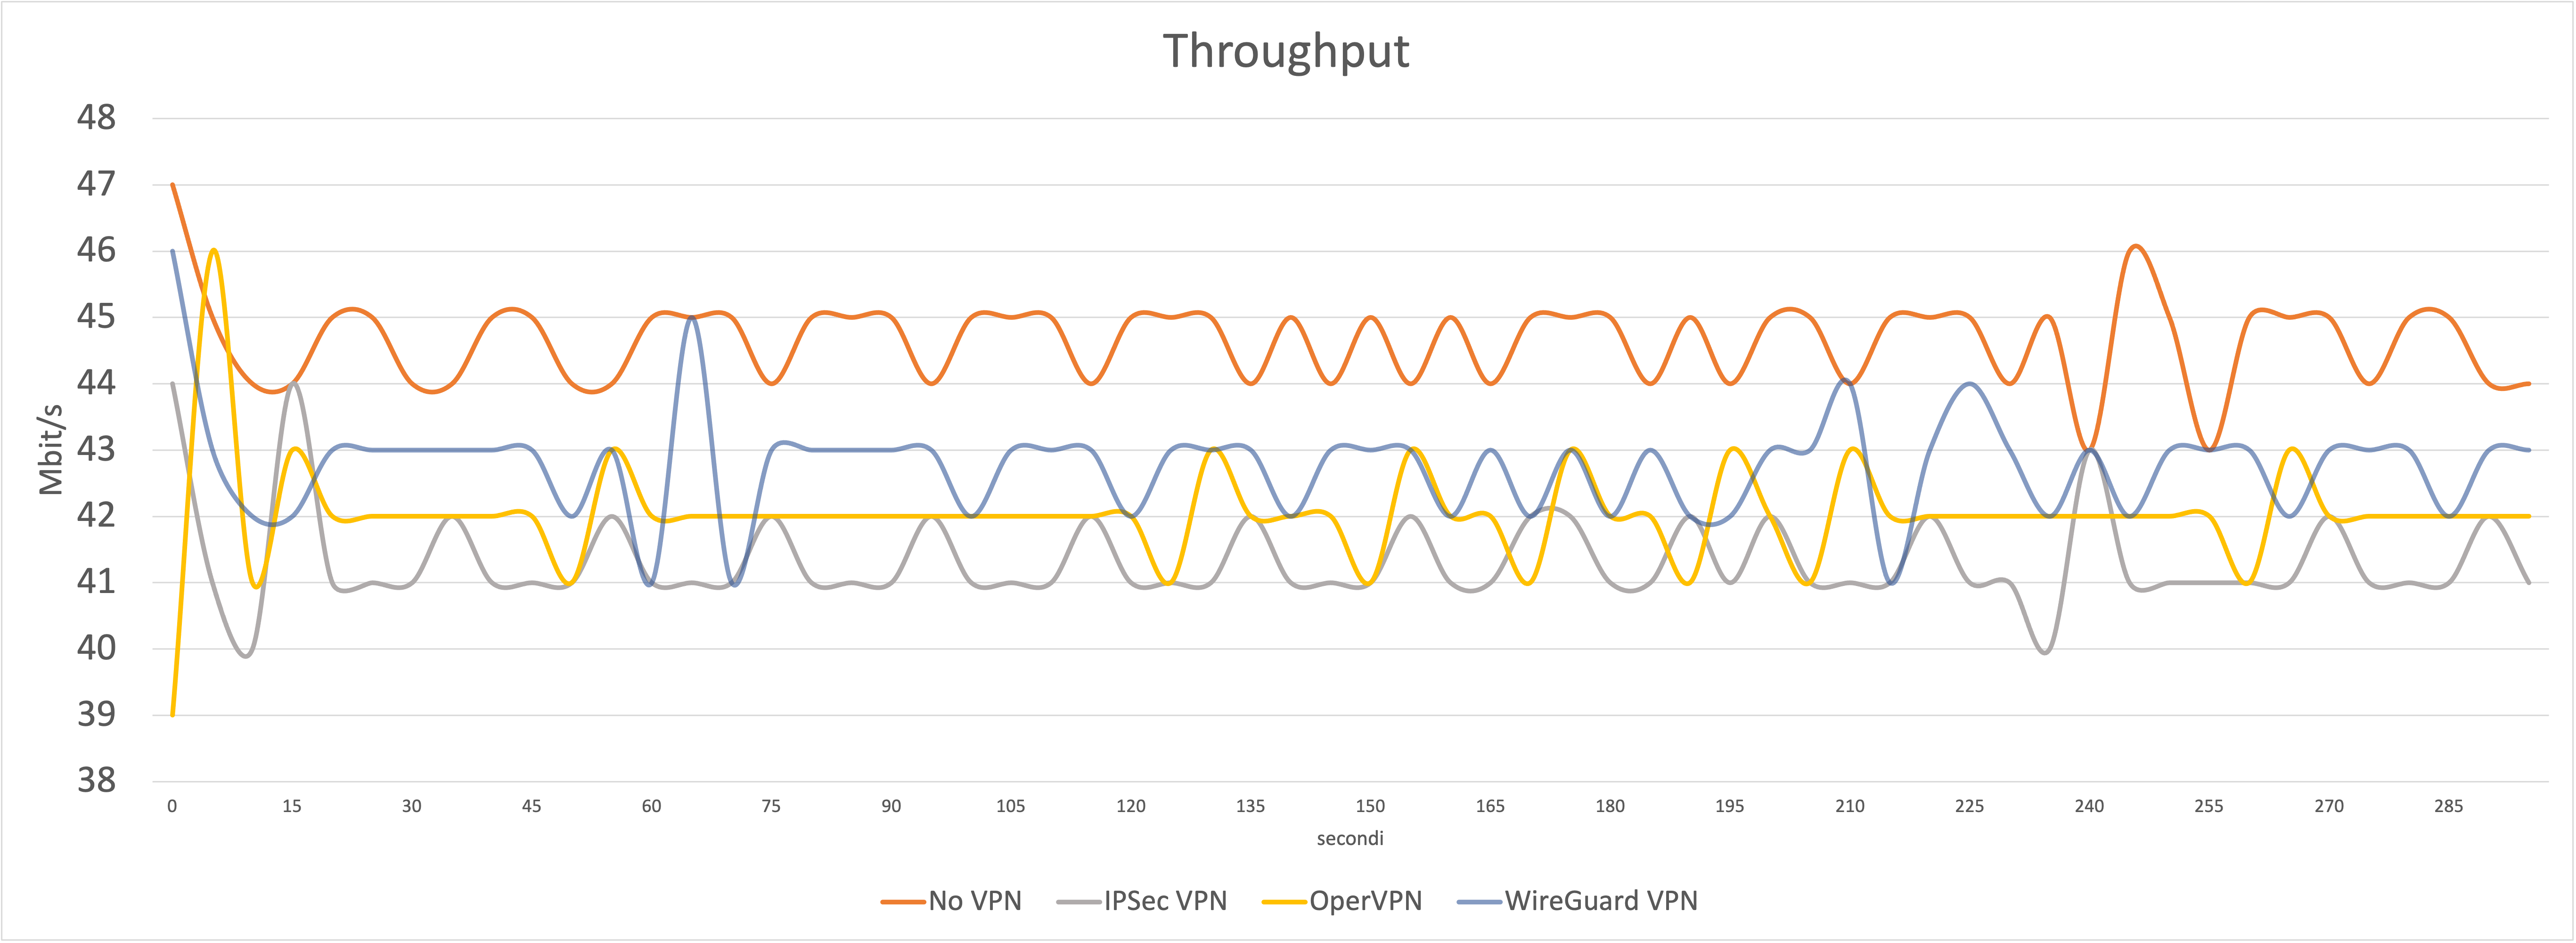
\includegraphics[width=14cm]{figure/fineThroughput.png}
    \caption{Confronto dei throughput raffinati}
\end{figure}

\begin{figure}[ht]
    \centering
    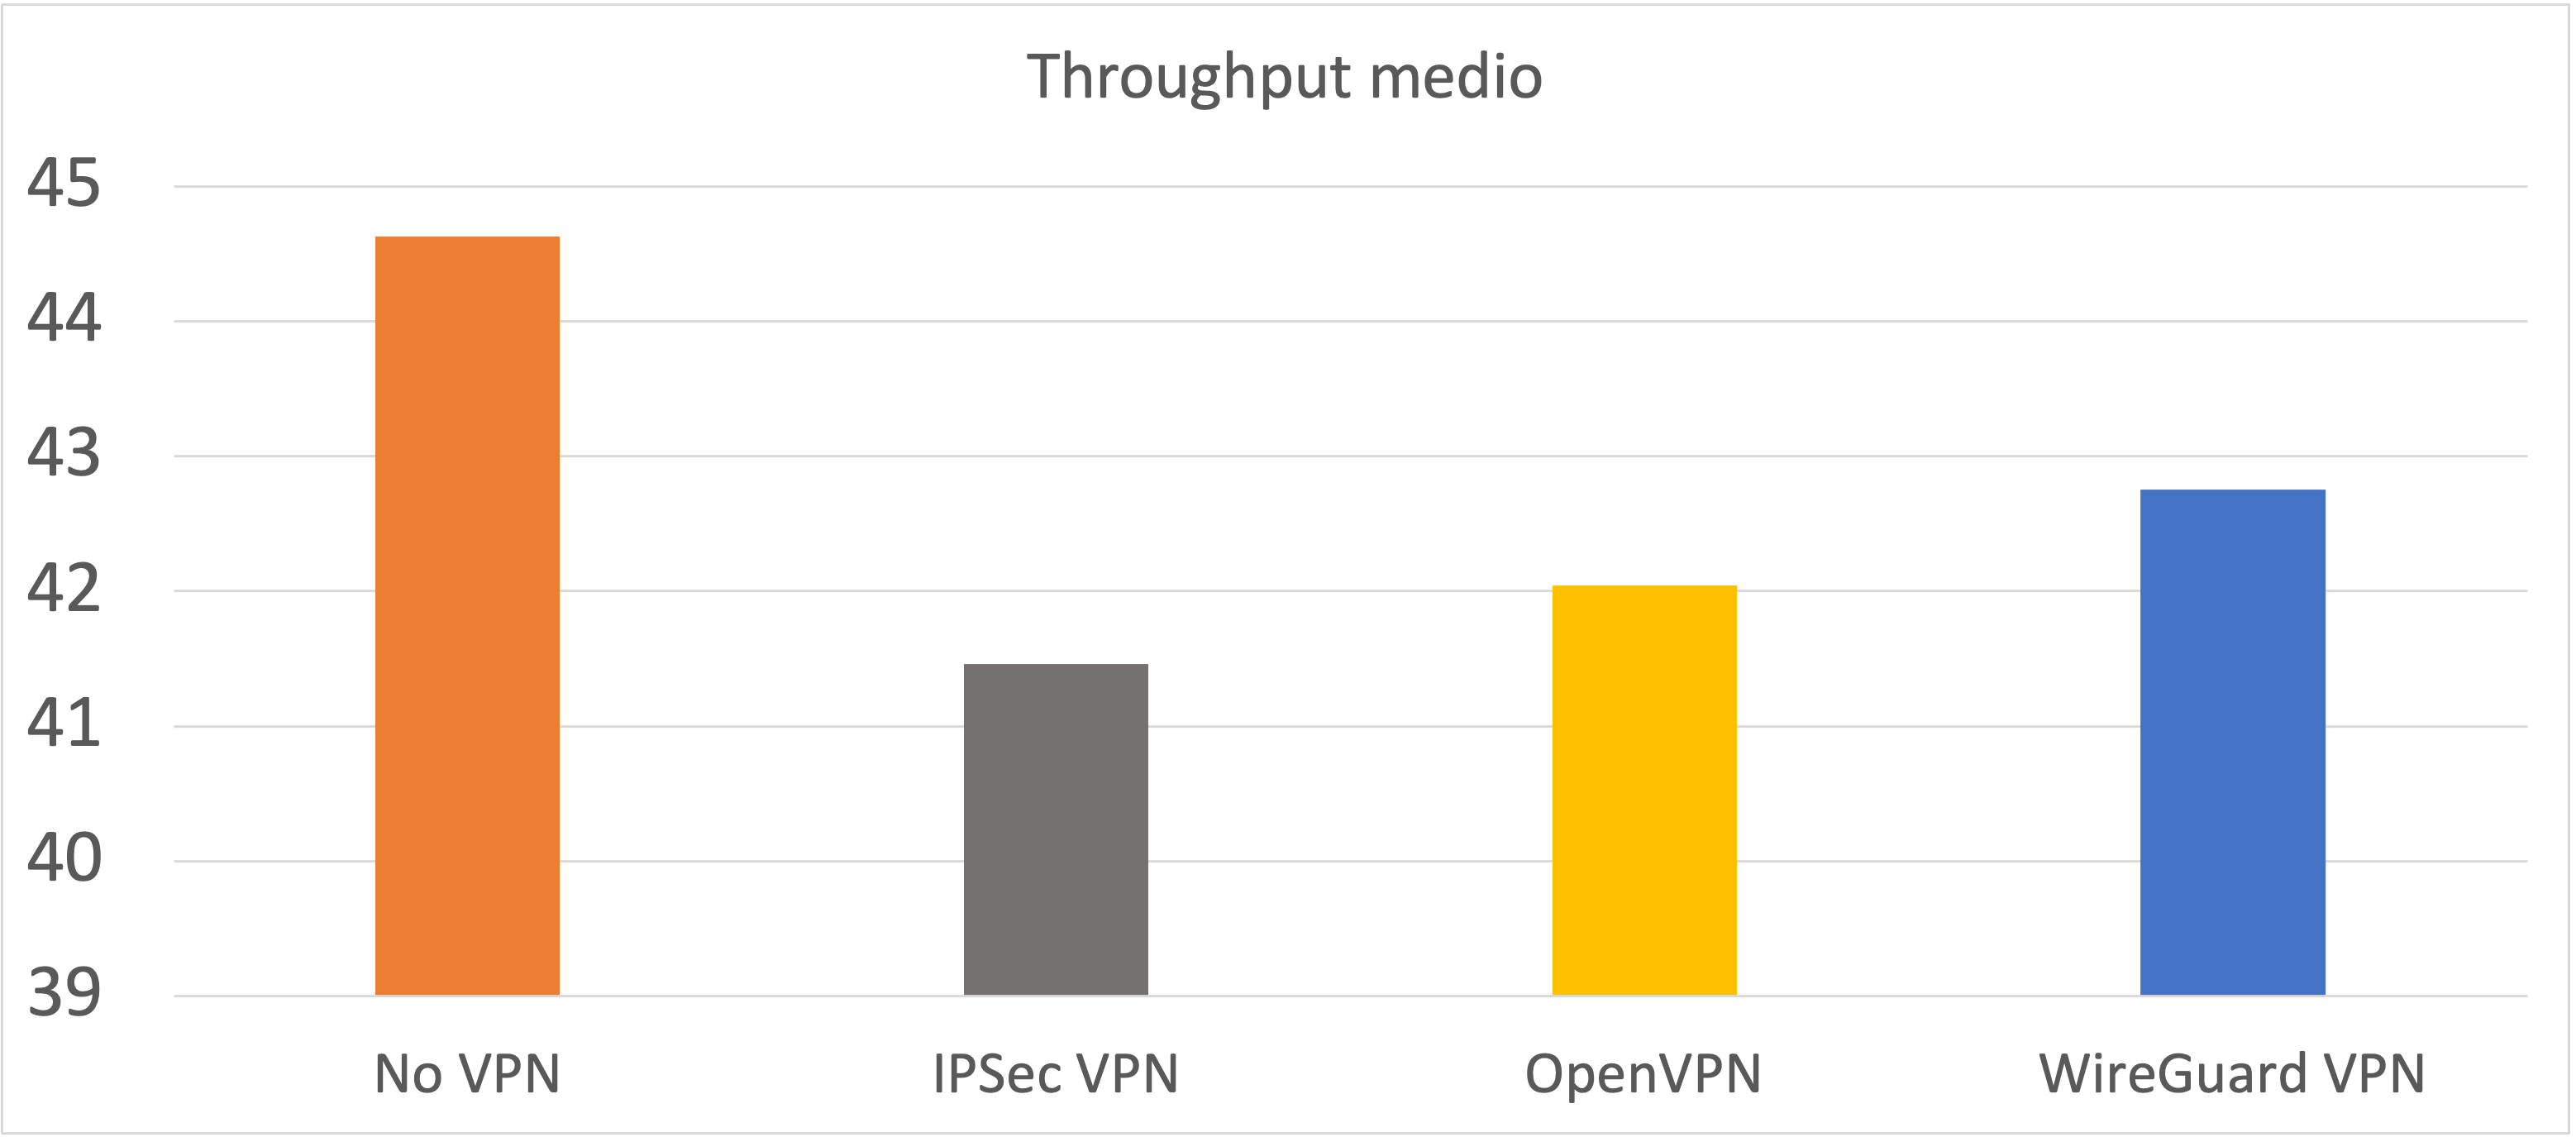
\includegraphics[width=10cm]{figure/avg.png}
    \caption{Confronto dei throughput medi}
\end{figure}